% Assignment 1 research report. Build from assignment1/report/ with:
%   tectonic -X compile main.tex
% Tables and figures are read from ../analysis (generated by analysis/analyze.py).
\documentclass[11pt,a4paper]{article}

\usepackage[T1]{fontenc}
\usepackage{lmodern}
\usepackage{microtype}
\usepackage[margin=2.4cm]{geometry}
\usepackage{amsmath}
\usepackage{booktabs}
\usepackage{graphicx}
\usepackage{xcolor}
\usepackage{listings}
\usepackage[font=small,labelfont=bf]{caption}
\usepackage{subcaption}
\usepackage{enumitem}
\usepackage[hidelinks]{hyperref}
\usepackage{url}

\graphicspath{{../analysis/figures/}}
\newcommand{\tabledir}{../analysis/tables}
\newcommand{\repourl}{\url{https://github.com/Xami650/Individual-Assignments-Big-Data-ULPGC}}
\newcommand{\session}{\texttt{20261014-225910}}

\lstset{
  basicstyle=\ttfamily\footnotesize,
  columns=fullflexible,
  keepspaces=true,
  frame=single,
  framesep=3pt,
  rulecolor=\color{black!30},
  aboveskip=4pt,
  belowskip=2pt,
  showstringspaces=false,
}

\setlist{itemsep=2pt,topsep=4pt}

\title{\textbf{Assignment 1: Basic Matrix Multiplication in Python, Java and C}\\[4pt]
\large How Matrix Size Affects Runtime and Memory of the Triple-Loop Algorithm}
\author{Máximo Prosperi Reynoso\\[2pt]
\small BIG DATA, GCID, ULPGC\\
\small Individual Assignment 1, 2026--2027\\[2pt]
\small \repourl}
\date{15 October 2026}

\begin{document}
\maketitle

\begin{abstract}
\noindent
This study asks how the matrix size $n$ affects the runtime and peak memory of
the same basic triple-loop matrix multiplication (i-j-k order, double precision,
one thread) implemented in Python (CPython~3.13), Java (OpenJDK~25) and C (clang
\texttt{-O2}) on an Apple M4 laptop. Under a protocol declared in advance, the
three implementations multiply the same seeded inputs, with bitwise-identical
results. Only the kernel is timed, after warm-up, with five measured samples per
size from $n=64$ to $2048$, peak resident memory from \texttt{/usr/bin/time -l},
and a 120\,s budget per multiplication. Runtime grew faster than $n^3$ (log-log
slopes 3.44 for C, 3.39 for Java, 3.22 for Python): for C and Java the
instructions per inner iteration stayed constant, while the cycles per
iteration rose with $n$. CPython was
35 to 62 times slower than C, executed about 540 to 660 instructions per
iteration against 8, and timed out at $n=1536$. C and Java stayed within a factor
of 0.68 to 1.26 of each other, with no consistent winner. Above each runtime's
baseline, memory was about 8\,B per matrix element for C and Java and 40\,B for
Python. The conclusions apply only to the tested implementations, settings,
inputs and machine.
\end{abstract}

% ===========================================================================
\section{Introduction and objective}

Dense matrix multiplication is the reference problem of this course's four
assignments. The basic algorithm performs $n^3$ multiply-add steps for two
$n\times n$ matrices, so its operation count is known exactly. Its runtime on a
real machine also depends on the language runtime that executes the loops and on
how the memory hierarchy serves the data. This first study measures these
effects for the plain algorithm, before any optimisation. It provides the
baseline that the later assignments (optimised and sparse, parallel, and
distributed multiplication) will improve on.

\paragraph{Research question.} \emph{How does the matrix size $n$ affect the
runtime and the peak memory of the same basic triple-loop dense matrix
multiplication implemented in Python, Java and C on one fixed machine?} The
factor is $n$, the side length of square $n\times n$ inputs. The outcomes are the
kernel wall-clock time per multiplication and the peak resident set size of the
process.

\paragraph{Hypotheses.} The following predictions were recorded in the
protocol file, \texttt{config/bench.json}, before any benchmark was run. They are
predictions, not results, and Section~\ref{sec:discussion} tests them against the
data.
\begin{description}[leftmargin=2.2em,style=sameline]
  \item[H1] Runtime grows approximately as $n^3$ for every implementation
  (log-log slope close to 3). C and Java may exceed 3 at the larger sizes,
  because the column-wise walk over $B$ increasingly misses in cache and TLB.
  \item[H2] At every tested size, CPython is one to two orders of magnitude
  slower than C and Java. C and Java stay within a small constant factor of
  each other once the JVM has compiled the kernel.
  \item[H3] Peak memory grows approximately as $n^2$. C stays close to the
  $24n^2$ bytes of its three arrays, Java adds a roughly constant JVM overhead,
  and Python needs several times more per element because its lists store
  pointers to boxed float objects.
  \item[H4] The three implementations produce bitwise-identical results,
  because they perform the same IEEE-754 double operations in the same order.
\end{description}

% ===========================================================================
\section{Background and references}
\label{sec:background}

\paragraph{The algorithm and its memory access pattern.} The product
$C=AB$ is defined by $C_{ij}=\sum_{k=0}^{n-1}A_{ik}B_{kj}$. The basic
algorithm computes each entry with a loop over $k$ nested inside loops over $i$
and $j$, for $n^3$ multiplications and $n^3$ additions. In the i-j-k order, the
inner loop reads row $i$ of $A$ with unit stride but column $j$ of $B$ with a
stride of one full row. With row-major storage, consecutive accesses to $B$ are
$8n$ bytes apart. Once the cache lines that hold a column of $B$ no longer fit in
cache, almost every access to $B$ misses. Bryant and O'Hallaron analyse this case
and the other loop orders~\cite{bryant2016}. Drepper uses exactly this loop as
his example and reports that transposing $B$ first cut the cycle count by 76.6\%
for $1000\times1000$ matrices on an Intel Core~2~\cite{drepper2007}.
High-performance libraries go much further, blocking the computation for each
cache level and for the TLB~\cite{goto2008}. Such changes alter the
algorithm's memory behaviour, so they are excluded from this controlled baseline
and left for Assignment~2.

\paragraph{Floating-point arithmetic.} All implementations use IEEE-754
binary64 numbers, for which every addition and multiplication is correctly
rounded~\cite{ieee754}. Results can therefore be bitwise identical across
languages only if the operations and their order are the same. A fused
multiply-add rounds once instead of twice, so it changes the result. Clang may
fuse \texttt{s + a*b} within one C statement by default; the option
\texttt{-ffp-contract=off} disables this~\cite{clangmanual}. Java has used strict
IEEE semantics everywhere since JDK~17~\cite{jep306}, and CPython evaluates each
operator separately. Higham shows that for any summation order, an $n$-term dot
product computed in floating point has a forward error of at most
$\gamma_n\sum_k|x_k||y_k|$, with $\gamma_n=nu/(1-nu)$ and unit roundoff
$u=2^{-53}$~\cite[Secs.~3.1, 3.5]{higham2002}. Two correct results for the same
product can therefore differ elementwise by at most $2\gamma_n(|A||B|)_{ij}$.
This study uses that bound as its tolerance (Section~\ref{sec:correctness}).

\paragraph{Language runtimes.} CPython compiles Python source to bytecode and
executes it in an interpreter. Every float is a separate heap object, and every
list element is a pointer to one. Since version~3.11 the interpreter specialises
instructions for the types it observes~\cite{pep659}. The experimental JIT
compiler of CPython~3.13 is not part of the default build~\cite{pep744}, and the
interpreter used here has it disabled. Small objects such as floats come from the
\emph{pymalloc} allocator~\cite{pythonmemory}. The HotSpot JVM starts by
interpreting bytecode and compiles frequently executed methods with its tiered
just-in-time compilers, which are enabled by default~\cite{javacmd}. Its early
iterations are therefore slower than its steady state, which is why Java
benchmarks need warm-up and steady-state measurement~\cite{georges2007}.

\paragraph{Related measurements.} Leiserson et al.\ use the same triple loop to
illustrate performance engineering~\cite{leiserson2020}. For two $4096\times4096$
matrices on an 18-core Intel machine, they report that Java ran 10.8 times faster
than Python~2, and C 47 times faster than Python. That single-size measurement on
different hardware motivates this study but cannot be compared directly with
it. Here the comparison covers a range of sizes and adds memory.

% ===========================================================================
\section{Methodology}
\label{sec:method}

\subsection{Implementations}

Each language has a kernel function with the same loop nest, shown in
Fig.~\ref{fig:kernels}, and a driver program with a common command-line
interface. All three kernels use the i-j-k order and a scalar double
accumulator, assign every $C_{ij}$, and call no library routine. The kernels
differ only where the languages force them to.
\begin{itemize}
  \item \textbf{Python:} a list of $n$ row lists of Python \texttt{float} objects.
  Each access \texttt{a[i][k]} performs two list subscripts and yields a pointer
  to a boxed float. Intermediate results are float objects as well. Only the
  standard library is used.
  \item \textbf{Java:} \texttt{double[][]}, an array of references to $n$
  separately allocated row arrays of primitive doubles. Each row is contiguous,
  but rows are distinct heap objects with their own headers, and every access is
  bounds-checked unless the JIT can prove it safe.
  \item \textbf{C:} one contiguous row-major block of $n^2$ doubles from
  \texttt{malloc}, indexed as \texttt{M[i*n+j]}. The kernel is in its own
  translation unit and the build uses no link-time optimisation, so the
  repeated calls of a timed batch cannot be merged or removed.
\end{itemize}

\begin{figure}[t]
\centering
\begin{subfigure}[t]{0.48\linewidth}
\begin{lstlisting}[language=Python]
def multiply(a, b, c, n):
    for i in range(n):
        for j in range(n):
            s = 0.0
            for k in range(n):
                s += a[i][k] * b[k][j]
            c[i][j] = s
\end{lstlisting}
\caption{Python (\texttt{python/matmul.py})}
\end{subfigure}\hfill
\begin{subfigure}[t]{0.48\linewidth}
\begin{lstlisting}[language=Java]
for (int i = 0; i < n; i++) {
  for (int j = 0; j < n; j++) {
    double s = 0.0;
    for (int k = 0; k < n; k++) {
      s += a[i][k] * b[k][j];
    }
    c[i][j] = s;
  }
}
\end{lstlisting}
\caption{Java (\texttt{MatMul.multiply})}
\end{subfigure}

\medskip
\begin{subfigure}[t]{0.48\linewidth}
\begin{lstlisting}[language=C]
for (size_t i = 0; i < n; i++) {
  for (size_t j = 0; j < n; j++) {
    double s = 0.0;
    for (size_t k = 0; k < n; k++) {
      s += a[i * n + k] * b[k * n + j];
    }
    c[i * n + j] = s;
  }
}
\end{lstlisting}
\caption{C (\texttt{c/src/matmul.c})}
\end{subfigure}\hfill
\begin{subfigure}[t]{0.48\linewidth}
\begin{lstlisting}
LBB1_4:               ; inner k loop
  ldr  d1, [x0, x13, lsl #3]  ; A[i][k]
  ldr  d2, [x14]              ; B[k][j]
  fmul d1, d1, d2
  fadd d0, d0, d1             ; s += ...
  add  x13, x13, #1
  add  x14, x14, x9           ; += 8n bytes
  cmp  x3, x13
  b.ne LBB1_4
\end{lstlisting}
\caption{Inner loop of (c) as compiled (\texttt{make asm})}
\end{subfigure}
\caption{The three kernels. They share the loop order, the scalar accumulator
and the order of operations. The compiled C inner loop has 8 scalar
instructions with separate multiply and add: no fused multiply-add and no
vectorisation. Compiled with clang's default contraction instead, the same
source contains an \texttt{fmadd}.}
\label{fig:kernels}
\end{figure}

\subsection{Inputs}

Every implementation reads the same binary input files, so all three multiply
logically identical matrices. For each size, \texttt{scripts/gen\_inputs.py}
draws $A$ and then $B$ from NumPy's PCG64 generator~\cite{harris2020}, seeded
with \texttt{SeedSequence([2026, n])}. The values are uniform on $[-1,1)$ and
are stored as raw little-endian float64 in row-major order without a header. The
SHA-256 digest of every file is tracked in the repository and checked whenever
the files are regenerated, because NumPy does not guarantee the same random
stream across versions.

\subsection{Execution environment}

Table~\ref{tab:env} lists the machine and the software. These settings were
fixed for every run.

\begin{table}[t]
\centering
\caption{Execution environment and fixed settings of the reported session
(\session, recorded in \texttt{env.txt} before and after the session).}
\label{tab:env}
\small
\begin{tabular}{@{}lp{0.72\linewidth}@{}}
\toprule
Machine & MacBook Air (Mac16,13), fanless; 24\,GiB RAM; AC power, Low Power Mode off \\
CPU & Apple M4: 4 performance cores (L1d 128\,KiB each, 16\,MiB L2 shared) and
6 efficiency cores (L1d 64\,KiB, 4\,MiB L2); 10 logical processors; 128\,B cache
line; 16\,KiB pages \\
OS & macOS 26.6.2 (build 25G83), Darwin 25.6.0 \\
C & Apple clang 21.0.0; \texttt{-std=c17 -O2 -ffp-contract=off -Wall -Wextra}
(no \texttt{-ffast-math}, no \texttt{-march}) \\
Java & OpenJDK 25.0.2 (HotSpot 64-bit Server VM), Maven 3.9.12;
\texttt{java -Xmx4g}; defaults otherwise: G1 collector, tiered compilation,
4 compiler threads, 9 parallel and 2 concurrent GC threads \\
Python & CPython 3.13.9 (Anaconda build), JIT disabled, GIL enabled;
\texttt{python3 -u}; NumPy 2.3.5 only for inputs and the correctness reference \\
Threads & the kernel runs on one thread in every language; benchmark processes
never load NumPy, so no BLAS threads exist \\
Conditions & no thermal or performance warning recorded before or after the
session; load average 3.1 at the start and 3.4 at the end, with desktop
applications open \\
\bottomrule
\end{tabular}
\end{table}

\subsection{Correctness checks}
\label{sec:correctness}

Each language has its own unit tests: 16 in Python (pytest), 17 in Java
(JUnit~5) and 36 checks in C. They cover hand-computed $2\times2$, $3\times3$ and
$1\times1$ products, identity and zero matrices, the overwriting of a reused
output buffer, the binary I/O, and the driver's output contract. Each suite also
compares against a reference: an exact BigDecimal computation in Java, an exact
int64 computation on integer-valued inputs in C, and NumPy in Python.

Before benchmarking, \texttt{scripts/verify.py} ran every implementation through
its normal command line for $n\in\{1,2,3,10,64,100,256\}$ and three cases. The
random case multiplies the shared inputs and uses \texttt{numpy.matmul} as the
reference; NumPy serves only as a check and is not one of the compared
implementations. The identity case computes $AI$, whose exact answer is $A$, and
the zero case computes $A\cdot0$, whose exact answer is $0$. A result passes if
$|C_{ij}-R_{ij}|\le 2\gamma_n(|A||B|)_{ij}$ for every entry, with no absolute
term. The bound is scaled by $|A||B|$ and not by $|C|$, because entries of $C$
can approach zero through cancellation. A $|C|$-relative tolerance would then be
meaningless, whereas the $|A||B|$ bound also covers exact zeros. The script also
checks whether the three outputs are bitwise identical (H4). During the
benchmark, every sample prints the sum of all entries of $C$, which consumes the
result and is compared across languages.

\subsection{Measurement protocol}
\label{sec:protocol}

\paragraph{Timer boundary.} Only the kernel is timed. Input loading, output
allocation and runtime start-up are outside the timed region. The clocks are
monotonic: \texttt{time.perf\_counter\_ns()} in Python, \texttt{System.nanoTime()}
in Java and \texttt{clock\_gettime(CLOCK\_MONOTONIC\_RAW)} in C.

\paragraph{Samples.} Each (language, $n$) configuration runs in one fresh
process, which performs its warm-up and then five measured samples on the same
input. Warm-up continues until at least 1\,s of warm-up work has run, with a
minimum of one sample (two for Java). A sample times $k$ back-to-back
multiplications and records $k$, so the time per multiplication is the elapsed
time divided by $k$. The first warm-up uses $k=1$. Every later sample uses
$k=\max(1,\lceil 0.1\,\text{s}/t\rceil)$, where $t$ is the time per multiplication
of the most recent warm-up, so short configurations are batched into samples of
about 0.1\,s. All measured samples of a configuration share the same $k$.
Warm-up samples are kept in the raw data but excluded from every summary.
The summaries report the median and the interquartile range (IQR, quartiles with
linear interpolation) of the five measured samples.

\paragraph{Run order and budgets.} The harness \texttt{scripts/run\_benchmarks.py}
ran $n=1$ (memory baseline) and then
$n\in\{64,128,256,384,512,768,1024,1536,2048\}$ in ascending order, with the
languages in the order C, Java, Python and a 2\,s pause between processes. The
sizes 384, 768 and 1536 sit between the powers of two, so that effects specific
to power-of-two strides can be told apart from the general trend. Each process
had 20\,s to load its inputs and then at most 120\,s for every sample. A process
that missed a deadline was killed and recorded as a timeout, and the larger sizes
for that language were skipped. The memory budget was 4\,GB of peak RSS, checked
after each run, and the session budget was 60\,min.

\paragraph{Memory metric and process counters.} Every process ran under
\texttt{/usr/bin/time -l}, which reports the process resource usage. The memory
metric is the \emph{peak resident set size} (maximum RSS) of the whole process,
measured identically for the three languages. It includes the runtime itself, so
the $n=1$ run gives each language's baseline, and the theoretical reference is
the $24n^2$ bytes of three float64 arrays. The same tool reports the
instructions retired and the cycles elapsed by the process. These counters were
divided by the total number of inner iterations the process executed (all
multiplications, warm-ups included, times $n^3$). Across all configurations, the
timed kernel accounted for 97 to 101\% of the process's user CPU time, so the
per-iteration values describe the kernel.

\paragraph{Protocol amendments.} Smoke tests before the reported session led to
two changes, both recorded in the protocol file. First, batch sizes were too
small for Java, because $k$ was calibrated on the first, interpreted run (at
$n=64$, 0.52\,ms against 0.09\,ms once compiled). The batch size is now re-calibrated on every warm-up sample (commit
\texttt{58c80d3}). Second, the first 0.2 to 0.3\,s of a process ran slower,
consistent with the CPU frequency ramp of macOS. For example, C at $n=128$ took
1.42, then 0.93, then a steady 0.84\,ms. The minimum of 1\,s of warm-up work was
added for this reason (commit \texttt{fd6fd3a}). No change was made after the
reported session.

% ===========================================================================
\section{Results}
\label{sec:results}

The reported session (\session) ran on 14 October 2026 and took 13.3 minutes.
The correctness results come from \texttt{scripts/verify.py}. Every other number
below is computed from the committed raw data by \texttt{analysis/analyze.py}.

\subsection{Correctness}

All unit tests passed. All 63 cross-language checks (7 sizes, 3 cases, 3
languages) were within the tolerance. The largest ratio of observed error to
bound was 0.126 (random case, $n=3$), falling to 0.0031 at $n=256$. The identity
and zero cases were exact at every size. At every verified size, the three
implementations produced bitwise-identical outputs. In the benchmark, the
checksums of all languages that completed a size were also identical for every
$n$ up to 2048.

\subsection{Runtime}

Table~\ref{tab:time} and Fig.~\ref{fig:time} give the median time per
multiplication. Variability was low. The IQR was at most 2.8\% of the median in
every configuration except Python at $n=256$ (4.8\%) and $n=1024$ (5.1\%). At
$n=1024$, the five Python samples drifted upward in run order (34.5, 34.6, 35.1,
37.7 and 36.4\,s).

\begin{table}[t]
\centering
\caption{Median kernel time per multiplication in milliseconds, with the IQR as
a percentage of the median in parentheses. Five measured samples per
configuration; warm-ups excluded.}
\label{tab:time}
\small
\input{\tabledir/tab_time.tex}
\end{table}

\begin{figure}[t]
\centering
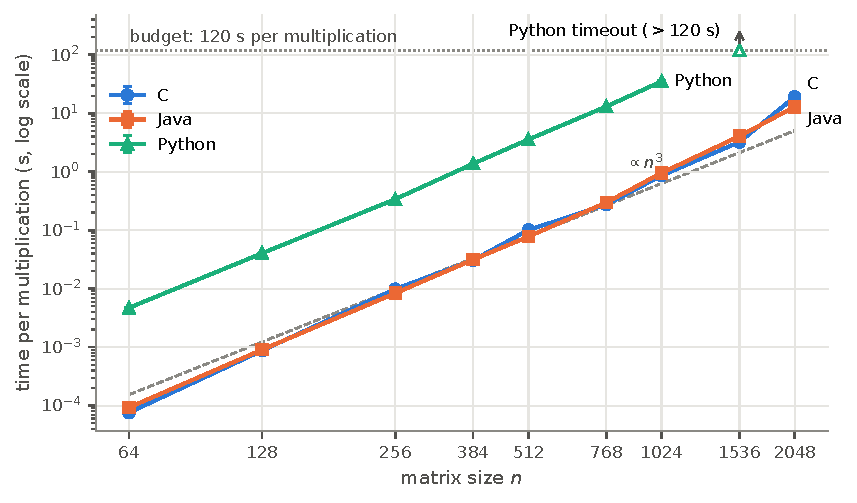
\includegraphics[width=0.80\linewidth]{fig_time.pdf}
\caption{Median kernel time per multiplication against $n$ (log-log). Error
bars show the IQR of five samples and are smaller than the markers. The dashed
line is proportional to $n^3$ and passes through the C median at $n=256$. The
open marker shows the Python timeout at $n=1536$ (budget 120\,s).}
\label{fig:time}
\end{figure}

\subsection{Growth with $n$}

If each inner iteration had a constant cost, the time divided by $n^3$ would be
flat. Fig.~\ref{fig:cost} and Table~\ref{tab:cost} show that it rose in every
language. From the smallest to the largest completed size, it grew 7.7-fold for
C (0.290 to 2.22\,ns), 4.2-fold for Java (0.355 to 1.50\,ns) and 1.8-fold for
Python (18.0 to 32.7\,ns). Table~\ref{tab:growth} gives the local growth exponents between consecutive
sizes and a global log-log fit. The global slopes are 3.44 for C, 3.39 for Java and
3.22 for Python. The local exponents of C are irregular, ranging from 2.47 to
4.14 up to $n=1536$, and reach 6.18 between 1536 and 2048. The cost per
iteration of C is lower at 384 than at 256 and 512, and lower at 768 than at 512
and 1024. Java's cost per iteration increased steadily at every step.

\begin{figure}[t]
\centering
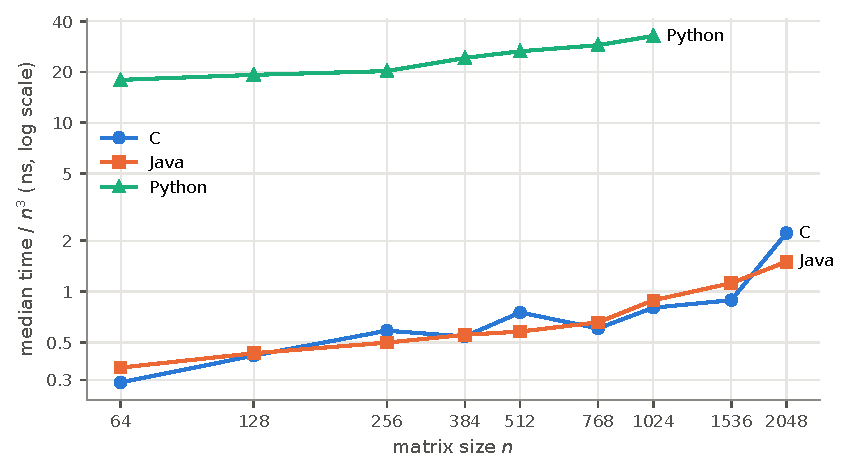
\includegraphics[width=0.74\linewidth]{fig_cost.pdf}
\caption{Median time per multiplication divided by $n^3$, i.e.\ the cost of one
inner-loop iteration, against $n$. A constant cost would be a horizontal
line.}
\label{fig:cost}
\end{figure}

\begin{table}[t]
\centering
\caption{Median time per inner iteration (time per multiplication divided by
$n^3$, in ns) and ratios of the median times to C.}
\label{tab:cost}
\small
\input{\tabledir/tab_cost.tex}

\bigskip
\caption{Local growth exponents $\log(t_2/t_1)/\log(n_2/n_1)$ between
consecutive sizes, and the slope of a least-squares fit of $\log t$ against
$\log n$ over all completed sizes.}
\label{tab:growth}
\input{\tabledir/tab_growth.tex}
\end{table}

\subsection{Cross-language comparison and process counters}

Fig.~\ref{fig:ratio} shows the time ratios to C. Python was 34.5 to 62.0 times
slower than C. The Java/C ratio ranged from 0.676 to 1.26. Java was faster than
C at $n=256$, 512 and 2048 and slower at the other six sizes.

Table~\ref{tab:counters} separates how much work each iteration does from how
long it takes. The instructions per inner iteration were essentially constant
in $n$ for C (8.0, exactly the length of the compiled loop in
Fig.~\ref{fig:kernels}d) and for Java (11.9 to 13.1). For Python they were 539
to 659. The cycles per iteration rose with $n$: from 1.19 to 8.93 for C, from
1.48 to 6.07 for Java and from 74 to 133 for Python. Dividing each process's
cycles by its user CPU time gives between 3.95 and 4.08 billion cycles per
second in every configuration.

\begin{figure}[t]
\centering
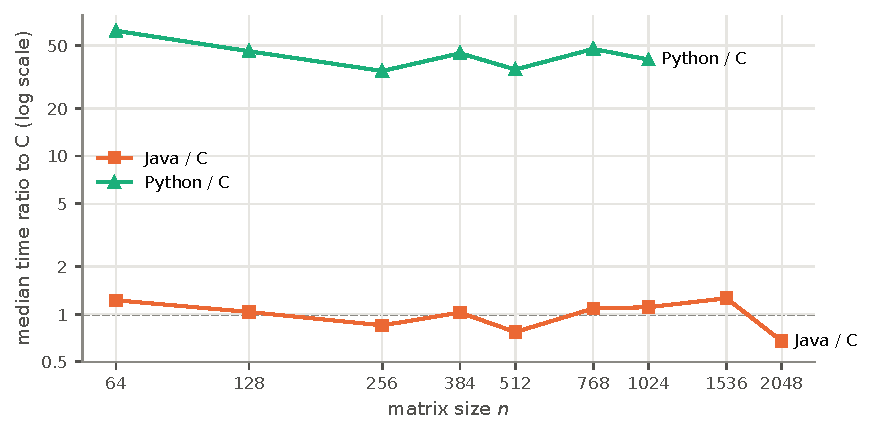
\includegraphics[width=0.72\linewidth]{fig_ratio.pdf}
\caption{Ratio of the median time per multiplication to that of C, at each $n$
(log scale; the dashed line marks parity).}
\label{fig:ratio}
\end{figure}

\begin{table}[t]
\centering
\caption{Instructions retired and cycles elapsed per inner-loop iteration,
from the process-wide counters of \texttt{/usr/bin/time -l}, divided by all
$n^3$ iterations the process executed (warm-ups included).}
\label{tab:counters}
\small
\input{\tabledir/tab_counters.tex}
\end{table}

\subsection{Memory}

Table~\ref{tab:memory} and Fig.~\ref{fig:memory} give the peak RSS. The $n=1$
baselines were 1.33\,MiB for C, 44.0\,MiB for Java and 13.7\,MiB for Python.
Fig.~\ref{fig:memory}b divides the peak RSS above the baseline by the $3n^2$
matrix elements. C used 8.0 to 8.2\,B per element at every $n\ge256$, and its peak RSS
at $n=2048$ was 97.4\,MiB against 96.0\,MiB for the three arrays. Python used
39.1 to 40.1\,B per element. Java used 8.2 to 10.5\,B per element, except for
14.1\,B at $n=1536$. That value comes from a jump of the peak RSS from 69.1\,MiB
at $n=1024$ to 139\,MiB, after which it reached only 143\,MiB at $n=2048$. From
$n=768$ upward, Python's peak RSS exceeded Java's despite the JVM baseline.

\begin{table}[t]
\centering
\caption{Peak resident set size of the whole process in MiB
(\texttt{/usr/bin/time -l}), with the storage of three float64 arrays for
reference.}
\label{tab:memory}
\small
\input{\tabledir/tab_memory.tex}
\end{table}

\begin{figure}[t]
\centering
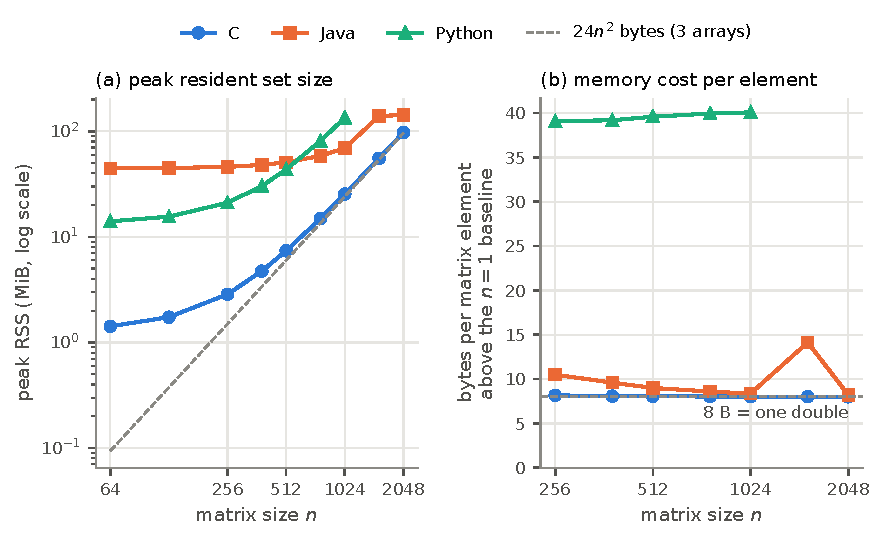
\includegraphics[width=0.86\linewidth]{fig_memory.pdf}
\caption{(a) Peak RSS against $n$ (log-log); the dashed line is $24n^2$ bytes.
(b) Peak RSS above the $n=1$ baseline divided by the $3n^2$ matrix elements, for
$n\ge256$ (at smaller $n$ the matrices are too small to separate from noise in
the runtime's own memory).}
\label{fig:memory}
\end{figure}

\subsection{Limits}

The largest size that met the budget was $n=2048$ for C (19.1\,s per
multiplication) and for Java (12.9\,s), and $n=1024$ for Python (35.1\,s). The
largest size attempted was $n=2048$ for C and Java and $n=1536$ for Python. At
$n=1536$, Python's first warm-up multiplication did not finish within 120\,s, so
the process was stopped and recorded as a timeout without any time, and $n=2048$
was skipped for Python. No configuration came near the memory budget: the
largest peak RSS was 143\,MiB, for Java at $n=2048$. Sizes above 2048 were not
attempted. At the cost per iteration measured for C at $n=2048$, a single
multiplication at $n=4096$ would already exceed the 120\,s budget.

% ===========================================================================
\section{Discussion}
\label{sec:discussion}

\paragraph{Answer to the research question.} On this machine, the runtime of
all three implementations grew faster than $n^3$ over the tested range. The
growth came from a rising cost per inner iteration. For C and Java, this was not
more work per iteration but more cycles for the same instructions. For Python,
the instructions per iteration also rose by about 20\%, for reasons not
investigated here, which accounts for part of its 1.8-fold increase. The
language set the level of the cost per iteration: CPython's iterations were
35 to 62 times more expensive than C's, while C and Java iterations cost
about the same. Peak memory grew as $n^2$ above a language-specific baseline.
The bytes per element were about 8 for C and Java and 40 for Python.

\paragraph{H1: growth against the cubic model.} Partially supported. Every
implementation follows the $n^3$ trend to first order (Fig.~\ref{fig:time}), but
all global slopes exceed 3, Python's included. The counters locate the cause.
C retires exactly 8 instructions per iteration at every size, so its work is
precisely cubic, yet its cycles per iteration grow 7.5-fold. The extra cycles
are therefore stall cycles, in which the processor waits instead of retiring
instructions. This is what the i-j-k access
pattern predicts: the inner loop walks a column of $B$ with a stride of $8n$
bytes~\cite{bryant2016,drepper2007}. The sizes give a rough scale for this
effect. One $B$ column occupies $n$ cache lines of 128\,B, which is
$128n$ bytes, so it reaches the size of the 128\,KiB L1d at $n=1024$. At
$n=2048$, each row of $B$ is exactly one 16\,KiB page, so one column walk
touches 2048 different pages. These calculations point to cache and TLB pressure, but this
study did not measure cache or TLB misses. The 6.18 exponent of C between 1536
and 2048 therefore remains unexplained beyond this general mechanism. Python's
slope (3.22) is the closest to 3: its cost per iteration rose only 1.8-fold.
This is consistent with the interpreter's fixed work per iteration being much
larger than the memory delays.

\paragraph{H2: interpreter and runtime effects.} Supported for Python, and
supported for Java versus C. CPython was 35 to 62 times slower than C, within
the predicted one to two orders of magnitude, and the counters explain most of
the gap. Each Python iteration executes about 540 to 660 machine instructions,
against 8 in C. These instructions perform bytecode dispatch, type checks, two
list subscripts per matrix access and the handling of float objects for the
intermediate results. The Python/C ratio was largest at $n=64$ (62.0), where C
ran at its lowest cost per iteration. It was lower (34.5 to 47.6) at every larger
size, where memory delays slowed C proportionally more than Python. For comparison, Leiserson et al.\ report a factor of 47 at $n=4096$
between Python~2 and C on an Intel server~\cite{leiserson2020}. This study's
range of 35 to 62 contains that value, but the interpreter versions and the
hardware differ.

After warm-up, Java stayed within a factor of 0.68 to 1.26 of C. Its
JIT-compiled loop retired about 12 instructions per iteration against 8 for C,
probably for bounds checks and row loads; the JIT output was not inspected.
At $n=256$, 512 and 2048, Java was still faster despite executing 50 to 60\%
more instructions, so at those sizes it must have lost fewer cycles to stalls. A
plausible explanation is the storage layout. At those three sizes, C's stride
through $B$ is an exact power of two, $8n$ bytes, which can concentrate the
column on a few cache sets. Java's rows are separate objects with headers, so
their spacing is not an exact power of two. The steady growth of Java's cost per
iteration fits this explanation. However, at $n=1024$, also a power of two, C
was faster than Java, which the explanation does not predict. The hypothesis
therefore stays open: testing it would require cache-miss counters or a padded C
layout. No general ranking of Java and C follows from these data.

\paragraph{H3: memory.} Supported, with a quantitative explanation for each
language. Above its 1.33\,MiB baseline, C uses 8.0 to 8.2\,B per matrix element:
the three arrays and almost nothing else. Java's large-$n$ values of 8.2 to 8.4\,B per
element match its \texttt{double[][]} payload plus small row headers, on top of
a 44\,MiB runtime baseline. The outlier at $n=1536$ coincides with the jump of
peak RSS described in the Results. This is consistent with the heap growing in
large steps, but heap use was not recorded, so the cause is not confirmed.
Python's 39 to 40\,B per element matches the storage of a float object plus a
list pointer. \texttt{sys.getsizeof(1.0)} reports 24\,B per float, but pymalloc
serves floats from 32-byte blocks: after one million floats were created,
\texttt{sys.\_debugmallocstats()} showed 1\,000\,639 blocks in use in the
32-byte size class. Adding the 8\,B pointer in the row list gives 40\,B per
element, which matches the measurement. As predicted, Python's per-element cost
is five times C's, which outweighs the JVM baseline from $n=768$ upward.

\paragraph{H4: identical results.} Supported. All three implementations
produced bitwise-identical matrices at every verified size and identical
checksums at every benchmarked size. This holds only because no implementation
fuses or reorders operations. The C build needs \texttt{-ffp-contract=off}
for this: with clang's default setting, the kernel compiles to a fused
multiply-add.

\paragraph{Limitations.}
\begin{itemize}
  \item \textbf{One machine, one session.} Each configuration has five samples
  from a single session. The IQRs describe the variability within that session,
  not between sessions or between machines.
  \item \textbf{Uncontrolled background load.} Desktop applications remained
  open (load average 3.1 to 3.4). macOS offers no user-level way to pin a
  thread to a performance core. The stable rate of about 4.0 billion cycles per
  second of CPU time suggests no large frequency drop, but the drift of the
  Python samples at $n=1024$ shows that the conditions were not perfectly
  constant.
  \item \textbf{Fanless laptop.} No thermal warning was recorded before or after
  the session, but no temperature was recorded during the runs.
  \item \textbf{Memory metric.} Peak RSS covers the whole process lifetime,
  including runtime start-up and input loading. It is not the same as JVM heap
  use or Python object counts, and the Java value depends on the collector's
  heap sizing.
  \item \textbf{Process-wide counters.} Instructions and cycles cover the whole
  process, including warm-ups and, for Java, JIT and GC threads. The kernel's
  97 to 101\% share of user CPU time limits this effect but does not remove it.
  \item \textbf{Clock resolution.} The clocks used advance in steps of about
  42\,ns (a 24\,MHz timebase), which is negligible because every sample lasted at least about 0.1\,s.
\end{itemize}

% ===========================================================================
\section{Conclusions}
\label{sec:conclusions}

For the tested implementations, settings, inputs and machine, this study
establishes the following:
\begin{enumerate}
  \item The three triple-loop implementations are correct within the declared
  tolerance and produce bitwise-identical results, given the same operation
  order and no fused multiply-add.
  \item Runtime grows faster than the cubic operation count (log-log slopes of
  3.2 to 3.4 between $n=64$ and 2048). For C and Java the number of
  instructions per iteration is constant, so the extra growth comes from more
  cycles per iteration, which is consistent with the matrices outgrowing the
  caches.
  \item CPython is 35 to 62 times slower than C, mainly because it executes
  67 to 82 times more instructions per iteration. Within the 120\,s budget it
  reaches $n=1024$, while C and Java reach $n=2048$.
  \item C and Java perform within a factor of 0.68 to 1.26 of each other, and
  which one is faster depends on $n$.
  \item Above each runtime's baseline, peak memory is about 8\,B per matrix
  element for C and Java and 40\,B for Python. Java adds a constant baseline of
  about 44\,MiB.
\end{enumerate}
Three questions remain unresolved. The first is why Java beats C at some sizes
but not others. The second is what causes the large jump of C between $n=1536$
and 2048. The third is whether these effects persist across sessions and
machines. Answering them requires cache and TLB miss counters, a padded memory
layout and repeated sessions. Those experiments, and loop orders that walk $B$
along its rows, belong to Assignment~2.

% ===========================================================================
\section{References and materials}
\label{sec:materials}

\paragraph{Reproducibility materials.} All code, data and scripts are in the
directory \texttt{assignment1/} of the GitHub repository below, at the tag
\texttt{assignment1-v1.0}:
\begin{center}\repourl\end{center}
Its README
gives the exact build and run commands and the software versions. The materials
are:
\begin{itemize}
  \item \texttt{c/}, \texttt{java/} and \texttt{python/}: the three
  implementations, their tests and the build files (Makefile, Maven POM).
  \item \texttt{config/bench.json}: the declared protocol, read by every script.
  \item \texttt{scripts/}: input generation (\texttt{gen\_inputs.py}),
  correctness verification (\texttt{verify.py}), the benchmark harness
  (\texttt{run\_benchmarks.py}) and the environment snapshot.
  \item \texttt{data/checksums.sha256}: the digests of the inputs, which are
  regenerated in about one second instead of being stored.
  \item \texttt{results/correctness.csv}: the outcome of the correctness checks.
  \item \texttt{results/raw/\session/}: every raw sample, warm-ups included
  (\texttt{samples.csv}), one row per process with status, peak RSS and counters
  (\texttt{runs.csv}), the environment snapshot (\texttt{env.txt}) and the
  protocol used (\texttt{config.json}).
  \item \texttt{analysis/analyze.py}: the script that produces every table and
  figure in this report from the raw data. Run again on the same data, it
  reproduces them byte for byte.
\end{itemize}

The whole study is reproduced from \texttt{assignment1/} with:
\begin{lstlisting}
python3 scripts/gen_inputs.py && python3 scripts/verify.py
python3 scripts/run_benchmarks.py && python3 analysis/analyze.py
\end{lstlisting}
The three implementations sit side by side in one project, in a repository that
also holds the other course assignments. This is not the recommended practice
for multi-language software, where each implementation would be its own
project. It is done only to keep the whole class submission together.

\paragraph{Use of generative AI.} Claude Code (Anthropic, model Claude Opus~5.5)
was used as a programming and writing assistant. It helped plan the protocol,
draft and debug the implementations, tests, benchmark harness and analysis
scripts, review the figures, and draft and revise the text of this report. All
measurements were produced by running the code on the author's machine, and
every result in Section~\ref{sec:results} is computed from the committed data by
the scripts in the repository. Each cited source was checked against the original
publication or documentation. The author reviewed the code and the text and is
responsible for the work and its conclusions.

\renewcommand{\refname}{References}
\begin{thebibliography}{99}\raggedright
\small

\bibitem{bryant2016}
R.~E. Bryant and D.~R. O'Hallaron, \emph{Computer Systems: A Programmer's
Perspective}, 3rd~ed. Boston, MA, USA: Pearson, 2016, ch.~6.

\bibitem{drepper2007}
U.~Drepper, ``What every programmer should know about memory,'' Red Hat, Inc.,
Nov. 2007. [Online]. Available: \url{https://www.akkadia.org/drepper/cpumemory.pdf}

\bibitem{goto2008}
K.~Goto and R.~A. van~de Geijn, ``Anatomy of high-performance matrix
multiplication,'' \emph{ACM Trans. Math. Softw.}, vol.~34, no.~3, Art.~no.~12,
May 2008, doi: 10.1145/1356052.1356053.

\bibitem{ieee754}
\emph{IEEE Standard for Floating-Point Arithmetic}, IEEE Std 754-2019, 2019,
doi: 10.1109/IEEESTD.2019.8766229.

\bibitem{clangmanual}
LLVM Project, ``Clang compiler user's manual: \texttt{-ffp-contract}.''
Accessed: Oct.~15, 2026. [Online]. Available:
\url{https://clang.llvm.org/docs/UsersManual.html}

\bibitem{jep306}
J.~Darcy, ``JEP 306: Restore always-strict floating-point semantics,''
OpenJDK, delivered in JDK~17. Accessed: Oct.~15, 2026. [Online]. Available:
\url{https://openjdk.org/jeps/306}

\bibitem{higham2002}
N.~J. Higham, \emph{Accuracy and Stability of Numerical Algorithms}, 2nd~ed.
Philadelphia, PA, USA: SIAM, 2002.

\bibitem{pep659}
M.~Shannon, ``PEP 659 -- Specializing adaptive interpreter,'' Python Software
Foundation, Apr. 2021. [Online]. Available: \url{https://peps.python.org/pep-0659/}

\bibitem{pep744}
B.~Bucher and S.~Ostrowski, ``PEP 744 -- JIT compilation,'' Python Software
Foundation. Accessed: Oct.~15, 2026. [Online]. Available:
\url{https://peps.python.org/pep-0744/}

\bibitem{pythonmemory}
Python Software Foundation, ``Memory management,'' Python 3.13 documentation.
Accessed: Oct.~15, 2026. [Online]. Available:
\url{https://docs.python.org/3.13/c-api/memory.html}

\bibitem{javacmd}
Oracle, ``The java command,'' Java SE 25 \& JDK 25 documentation. Accessed:
Oct.~15, 2026. [Online]. Available:
\url{https://docs.oracle.com/en/java/javase/25/docs/specs/man/java.html}

\bibitem{georges2007}
A.~Georges, D.~Buytaert, and L.~Eeckhout, ``Statistically rigorous Java
performance evaluation,'' in \emph{Proc. 22nd Annu. ACM SIGPLAN Conf.
Object-Oriented Programming Systems, Languages and Applications (OOPSLA)},
2007, pp.~57--76, doi: 10.1145/1297027.1297033.

\bibitem{leiserson2020}
C.~E. Leiserson, N.~C. Thompson, J.~S. Emer, B.~C. Kuszmaul, B.~W. Lampson,
D.~Sanchez, and T.~B. Schardl, ``There's plenty of room at the Top: What will
drive computer performance after Moore's law?'' \emph{Science}, vol.~368,
no.~6495, Art.~no.~eaam9744, Jun. 2020, doi: 10.1126/science.aam9744.

\bibitem{harris2020}
C.~R. Harris \emph{et al.}, ``Array programming with NumPy,'' \emph{Nature},
vol.~585, no.~7825, pp.~357--362, Sep. 2020, doi: 10.1038/s41586-020-2649-2.

\end{thebibliography}

\end{document}
